% todo
%\section{基本命令}

\chapter{命令补充}


\section{打印系统相关的信息}
\begin{itemize}
\item 安装:
\begin{lstlisting}
# ubuntu 
$ sudo apt-get install -y screenfetch 

# opensuse 
$ sudo zypper in screenfetch
\end{lstlisting}

\item 运行:
\begin{lstlisting}
$ sudo screenfetch
\end{lstlisting}

% opensuse screenfetch  
% h: 当前位置(here)。将图形放置在正文文本中给出该图形环境的地方。如果本页所剩的页面不够,这一参数将不起作用。
% t: 顶部(top)。将图形放置在页面的顶部
% b: 底部(button)。将图形放置在页面的底部
% p: 独立一页(page)。将图形放置在一只允许有浮动对象的页面上。

\begin{figure}[htp]  
    \centering
    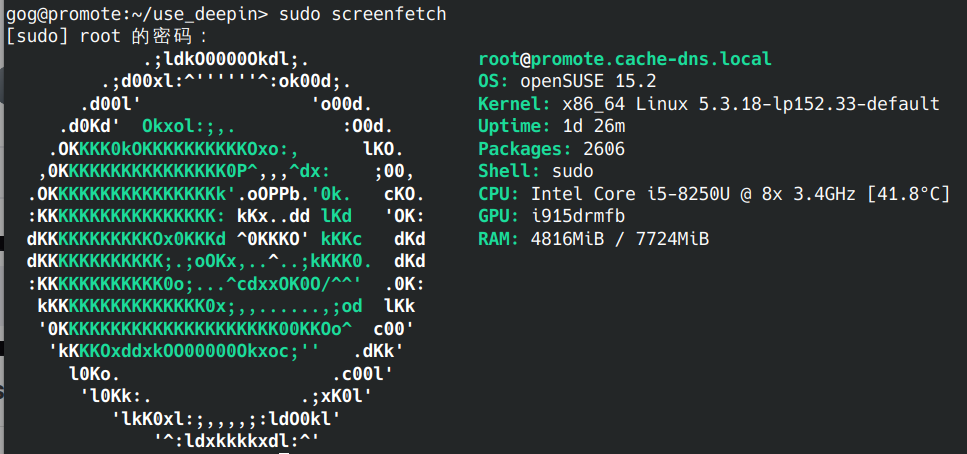
\includegraphics[width=0.49\textwidth]{./img/screenfetch/opensuse.png}
    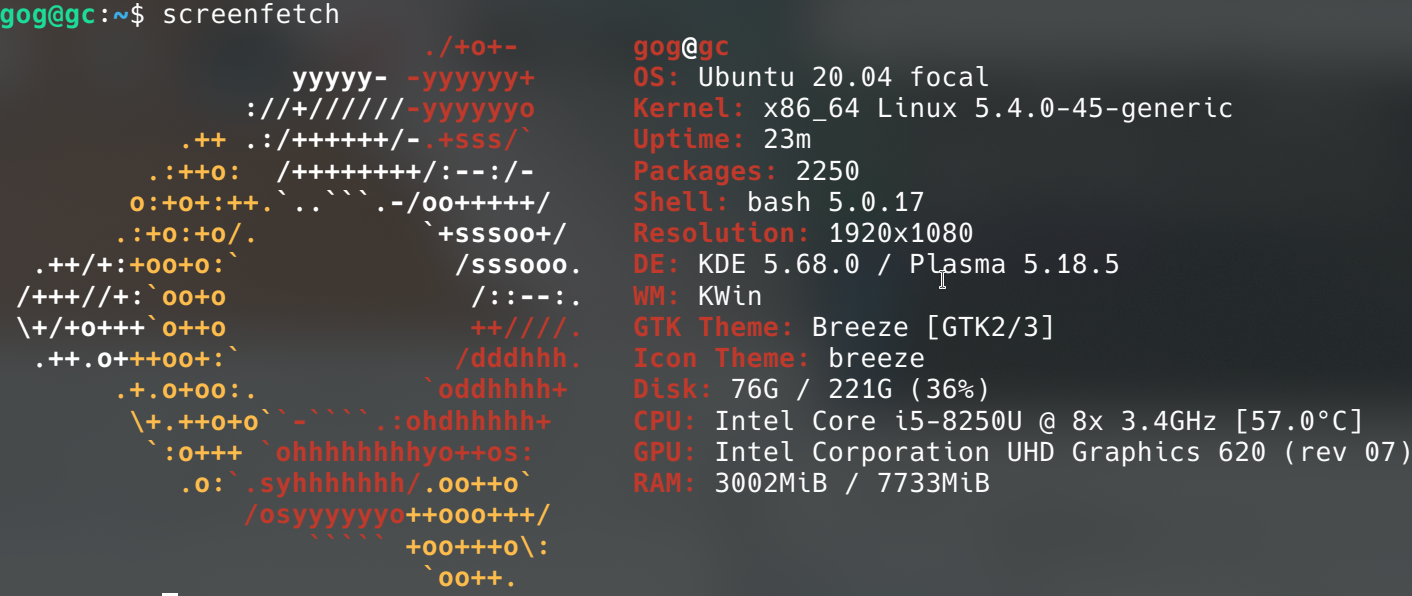
\includegraphics[width=0.49\textwidth]{./img/screenfetch/ubuntu.png}
    \caption{不同系统上的运行结果} %caption是图片的标题
    \label{fig:screenfetch} %此处的label相当于一个图片的专属标志,目的是方便上下文的引用
\end{figure}
\end{itemize}

% \section{make}
